%\documentclass[epsfig,a4paper,11pt,titlepage,twoside,openany]{book}
\documentclass[a4paper,12pt,titlepage,twoside,openany]{book}
\usepackage{epsfig}
\usepackage{plain}
\usepackage{setspace}
\usepackage[paperheight=29.7cm, paperwidth=21cm,outer=1.5cm,inner=2.5cm,top=2cm,bottom=2cm]{geometry} % per definizione layout
\usepackage{titlesec} % per formato custom dei titoli dei capitoli
\usepackage[utf8x]{inputenc} % supporto lettere accentate
\usepackage{graphicx}
\usepackage[italian]{babel}
\usepackage{verbatim}
\usepackage{amsmath}
\usepackage{amssymb} 
\usepackage{cite}  
\usepackage{mathtools} 	
\usepackage{microtype} 
\usepackage{listings}
\usepackage{subcaption} 				% enable subcaption (load also CAPTION)
	\captionsetup{font=small,labelsep=period,format=hang,tableposition=top,figureposition=bottom}
\usepackage[pdftex]{hyperref} 			% for interactive links
	\hypersetup{colorlinks=true,allcolors=black}

\singlespacing
\graphicspath{ {./images/} }

\begin{document}

% nessuna numerazione
\pagenumbering{gobble}
\pagestyle{plain}

\thispagestyle{empty}

\begin{center}
  \begin{figure}[h!]
    \centerline{
\psfig{file=marchio_unitrento_colore_it_202002.eps,width=0.6\textwidth}}
  \end{figure}

  \vspace{2 cm}

  \LARGE{Dipartimento di Ingegneria e Scienza dell’Informazione\\}

  \vspace{1 cm}
  \Large{Corso di Laurea in Informatica}

  \vspace{2 cm}
  \Large\textsc{Elaborato finale\\}
  \vspace{1 cm}
  \Huge\textsc{Titolo\\}
  \Large{\it{Sottotitolo (alcune volte lungo - opzionale)}}


  \vspace{2 cm}
  \begin{tabular*}{\textwidth}{ c @{\extracolsep{\fill}} c }
    \Large{Prof. Bouquet Paolo} & \Large{Corte Pause Manuela}\\
  \end{tabular*}

  \vspace{2 cm}

  \Large{Anno accademico 2021/2022}

\end{center}
\clearpage


% inizio numerazione pagine in numeri arabi
\mainmatter
%\pagestyle{fancy}
%\fancyhf{}
%\fancyhead[RO]{\leftmark}
%\fancyhead[LE]{\leftmark}
%\fancyfoot[C]{number}
%\fancypagestyle{plain}% you can add edits that won't affect "fancy" but only "plain"

% indice
\tableofcontents
\clearpage

% definizione titoli in forma "numero capitolo titolo capitolo"
\titleformat{\chapter}
{\normalfont\Huge\bfseries}{\thechapter}{1em}{}

\titlespacing*{\chapter}{0pt}{0.59in}{0.02in}
\titlespacing*{\section}{0pt}{0.20in}{0.02in}
\titlespacing*{\subsection}{0pt}{0.10in}{0.02in}
\titlespacing*{\subsubsection}{0pt}{0.10in}{0.02in}

% lista dei capitoli
\chapter{Introduzione}
\label{cha:intro}

I dati sono diventati una parte sempre più fondamentale della nostra vita e ancor di più in quella delle aziende nell'assisterle nel processo di decision-making.
Questi dati provengono da molteplici fonti come social network, online tracking, sensori di IoT, \dots e risultano in una mole enorme di dati non strutturati e
di conseguenza complessi da sfruttare per ricavarne informazioni rilevanti.
Proprio per questo il mondo della data integration è così importante \cite{DataIntegration}.

Possiamo definire la data integration come il problema del combinare dati provenienti da livelli diversi e fornire all'utente finale una 
visione unificata di questi\cite{dataIntegrationDef}. E' facile vedere quindi come questo concetto si adatti bene in un'azienda che utilizza vari sistemi, applicazioni 
e piattaforme ognuna delle quali produce o raccoglie dati senza tenere conto degli altri applicativi creando quelli che vengono definiti data silos.

Esistono approcci diversi alla data integration e quelle più tradizionale è certamente quello dei data warehouse, ovvero tutti i dati sono combinati e memorizzati in un solo posto (tipicamente un database). 
Questo processo di "combinazione" è definito ETL (Extract, Transform, Load) e permette di rilevare e correggere inconsistenze tra i dati prima che questi vengano uniti di questi. Inoltre permette di integrare 
tipi di dati eterogenei e visualizzarli poi come un'unica collezione complessiva.

Questa soluzione risulta complessa da utilizzare per dataset che vengono modificati frequentemente e richiedono quindi che il processo di ETL, che è molto costoso, venga re-eseguito molte volte.
Anche per questo si è quindi passati ad un paradigma basata sul \textit{loose coupling} ovvero si ha un'interfaccia sulla quale eseguire query che vengono poi mappate ed eseguite sulle sorgenti originali eliminando il 
problema dell'avere informazioni non aggiornate \cite{DataIntegrationHistory}. Questi due approcci sono descritti in figura \ref{fig:dataIntegration}.

\begin{figure}[ht]
    \centering
    \begin{minipage}{0.45\linewidth}
        \centering
        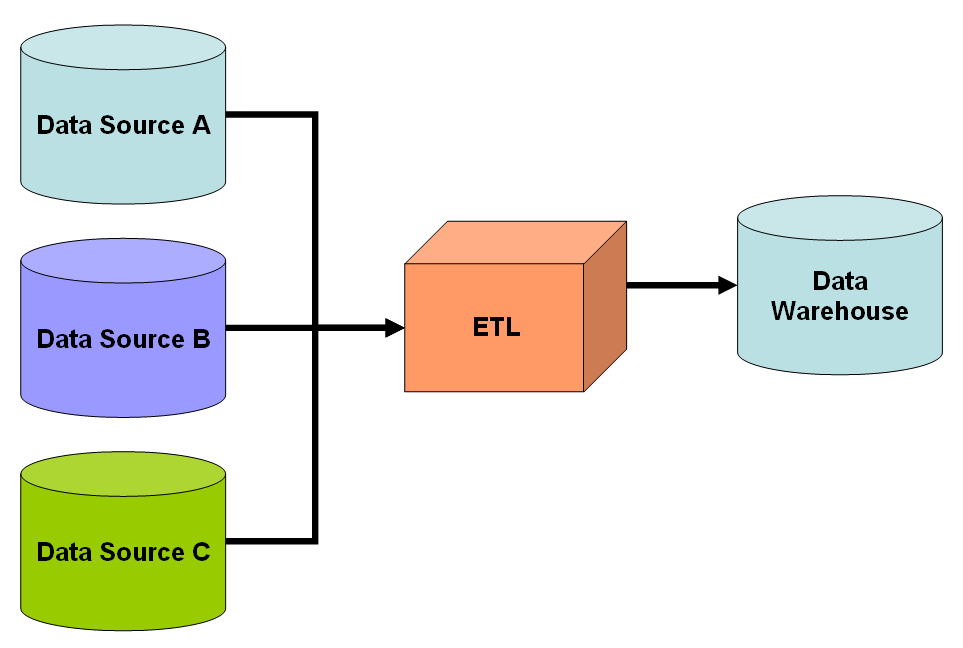
\includegraphics[width=0.9\linewidth]{Datawarehouse.png}
    \end{minipage}
    \begin{minipage}{0.45\linewidth}
        \centering
        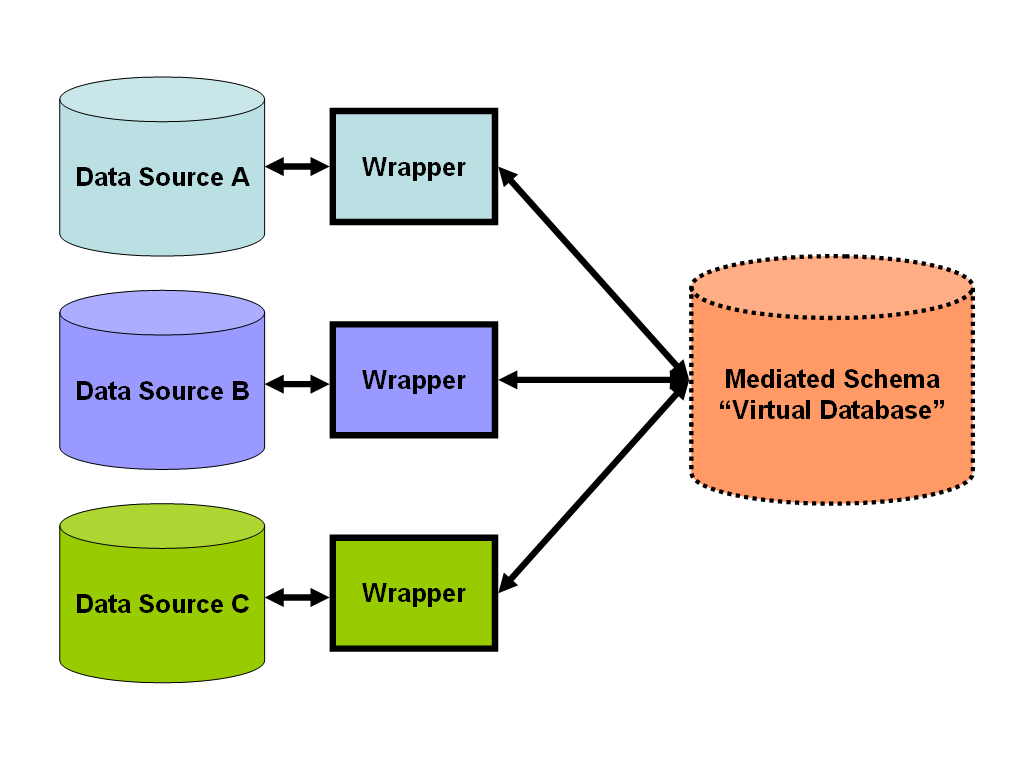
\includegraphics[width=0.9\linewidth]{Dataintegration.png}
    \end{minipage}
    \caption{Approcci alla data integration}
    \label{fig:dataIntegration}
\end{figure}
Indipendentemente dall'architettura del sistema, l'aspetto semantico risulta molto importante al fine di evitare la collisione tra termini uguali usati all'interno delle sorgenti con significati
diversi. \`E proprio da questa considerazione che nascono approcci basati su ontologie definiti come Ontology Based Data Access (OBDA). Queste soluzioni mitigano il problema appena descritto fornendo un vocabolario 
comune da utilizzare, ma presentano però il problema di essere complesse e di conseguenza poco fruibili da un ampio pubblico.

Lo scopo di questo elaborato è per prima cosa quello di descrivere i principali concetti teorici alla base delle ontologie e dei Knowledge Graph ed in particolare del Virtual Knowledge Graph system Ontop. Una volta stabilite delle
basi teoriche comuni verrà descritta l'esperienza di tirocinio da me svolta presso l'azienda Ontopic al fine di sviluppare un strumento che permetta l'interrogazione di un ontologia tramite strumenti di business intelligence 
come Tableau. In questo modo l'ontologia può essere interrogata anche da persone non esperte del campo dato che le query possono essere scritte in SQL o addirittura tramite l'interfaccia grafica fornita dagli strumenti di 
business intelligence.
\addcontentsline{toc}{chapter}{Sommario}
\chapter{Knowledge Graphs}
\label{cha:vkg}

\section{Cos'è un Knowledge Graph}
\label{sec:kg_description}

Si inizia a parlare di rappresentazione della conoscenza tramite l'aiuto di knowledge base già dalla fine degli anni 50 e nel 1980 ricercatori dell'università di Groningen 
e dell'università di Twente nei Paesi Bassi usarono per la prima volta il termine Knowledge Graph per descrivere il loro sistema basato sull'integrazione di molteplici sorgenti
di dati per rappresentare il linguaggio naturale tramite una knowledge base .
Questo primo momento di ricerca iniziale fu poi seguito all'inizio degli anni 2000 dall'affermazione degli standard W3C, come RDF e OWL, nell'ambito del 
Semantic Web a dal sorgere di varie ontologie pubbliche come DBPedia, YAGO e Freebase. \cite{KGDefinition} \cite{KGSurvey}

Il termine Knowledge Graph viene però diffuso solo nel 2012 con il motore di ricerca di Google che introduce il termine per descrivere
le nuove funzionalità di ricerca semantica del proprio motore di ricerca: le ricerche che vengono effettuate non sono più semplicemente string matching,
ma viene aggiunta una componente di ragionamento di grado di riconoscere veri e propri "oggetti" del mondo reale. \cite{KGDefinition}

La definizione precisa di cosa sia un Knowledge Graph rimane nebulosa e definizioni differenti risultano essere a volte in contraddizione l'una con l'altra. 
In modo molto generale possiamo definire un Knowledge Graph come una struttura che rappresenta la conoscenza come un insieme di concetti e le relazioni fra essi.
Se vogliamo invece dare una definizione più formale possiamo definire un knowledge graph come una struttura che acquisisce e integra informazioni in una knowledge base
e applica un motore d'inferenza per ricavare nuova conoscenza come mostrato in figura \ref{fig:KG}.
In molte delle definizioni la presenza di una quantità elevata di dati (un ABox di grandi dimensioni) viene spesso considerata un aspetto caratterizzante di un Knowledge Graph,
ma cosa significa nello specifico "quantità elevata" non è meglio specificato.

La knowledge base è tipicamente implementata tramite un'ontologia, ovvero una struttura a grafo dove i nodi rappresentano gli oggetti e i valori mentre le relazione tra questi 
e le loro proprietà sono rappresentate tramite archi. Questa rappresentazione tramite grafi permette una crescita più flessibile non avendo uno schema definito a priori ed è quindi adatto
per rappresentare domini complessi che attingono dati da fonti molteplici e diversificate tra di loro. Inoltre i linguaggi di interrogazione per strutture a grafo sono molto espressivi e 
contengono la maggior parte dei costrutti usati nei linguaggi di query più tradizionali come join, unioni, proiezioni, \dots \cite{KGIntro}.


\begin{figure}[ht]
    \centering
    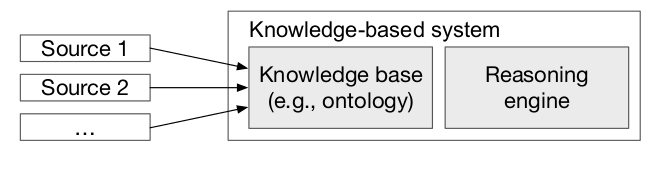
\includegraphics[width = 0.75\linewidth]{KG}
    \caption{Struttura di un KG}
    \label{fig:KG}
\end{figure}


\section{Virtual Knowledge Graph}
\label{sec:vkg_description}
I virtual knowledge graph applicano al concetto di knowledge graph quello di data virtualization. Questo significa che l'ontologia in un VKG l'ontologia non viene materializzata, ma viene dichiarato un insieme di mapping 
che permette di tradurre un insieme di concetti e proprietà tipiche di un'ontologia in un query SQL che vengono eseguite direttamente sulle sorgenti relazionali. 

Da un punto di vista più formale possiamo considerare la specifica di un Virtual Knowledge Graph come una tupla P = (O, M, S) dove abbiamo:
\begin{itemize}
    \item ontologia O: rappresentazione a grafo del dominio in analisi con un vocabolario rappresentativo del dominio. 
        In questo modo viene implementata una separazione tra i dettagli di basso livello delle fonti e la visione d'insieme data dall'ontologia che permette così anche a persone esperte nel campo, ma nell'integrazione 
        dei dati di ricavare informazioni. 
        In particolare W3C presenta vari standard per la rappresentazione delle ontologie tra cui i principali RDFS e OWL, entrambi basati sullo standard RDF (Resource Description Network) usato per descrivere grafi e al 
        fine di interrogare questo grafo lo standard è SPARQL.
    \item mapping M: insieme di affermazioni che specifica come le classi e le proprietà presenti nell'ontologia siano popolate da dati provenienti dalle sorgenti. Formalmente, dato lo schema di un database S e 
        un'ontologia O, un'affermazione di mapping tra S e O è un espressione in una di queste forme:
        \[ \phi(x) \leadsto (f(x) \ \textrm{rdf:type A}) \]
        \[\phi(x, x') \leadsto (f(x) \ P \ f'(x'))\] 
        dove $f$ è un costruttore di termini RDF ovvero una funzione che mappa una tupla di un database a una URI o un letterale RFD.
        In altre parole tutte le tuple del database vengono tradotte dando informazioni o sul tipo di dato o su relazioni di tipo (soggetto, predicato, oggetto)
        Lo standard per i mapping tra RDF e database relazionali fornito da W3C è R2RML.
    \item schema S: struttura delle sorgenti dati, tipicamente database relazionali.
\end{itemize}

A questo punto possiamo definire un'istanza di un Virtual Knowledge Graph come la coppia (P, D) dove P = (O, M, S) è la specifica di un VKG istanziata su un database D che rispetta lo schema S.
Dati M e D le triple generate applicando M su D costituiscono il grafo RDF che definisce il significato semantico dell'intero sistema.

Se vogliamo caratterizzare un Virtual Knowledge Graph sotto il punto di vista della logica descrittiva allora possiamo considerare l'ontologia come un TBox e le informazioni ricavate dalle sorgenti 
tramite i mapping come l'ABox \cite{OBDA} \cite{VKGOverview}. 


\begin{figure}[ht]
    \centering
    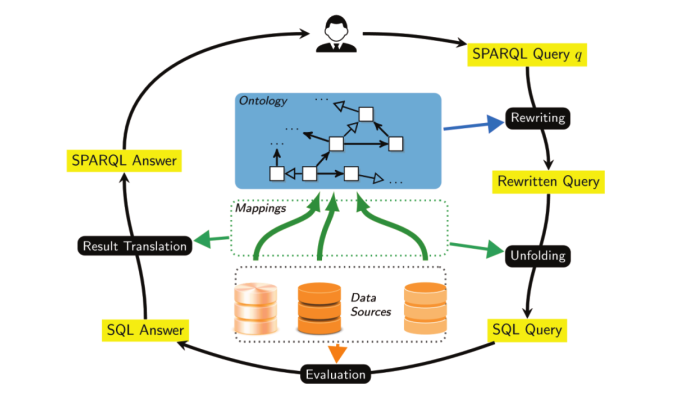
\includegraphics[width = 0.75\linewidth]{VKGRewriting.png}
    \caption{Riscrittura di una query in un VGK}
    \label{fig:VKGRewriting}
\end{figure}


\section{Il Virtual Knowledge Graph system Ontop}
\label{sec:vkg_ontop}
Ontop è un Virtual Knowledge Graph system open-source sviluppato dalla Libera Università di Bolzano e dall'azienda Ontopic s.r.l. . Riceve inoltre
contributi importanti da Birkbeck, University of London.

\subsection{Architettura del sistema}
Possiamo considerare Ontop come strutturato su quattro livelli e riassunto in figura \ref{fig:OntopArchitecture}
\subsubsection*{Input}
Ontop supporta gli standard W3C in materia di ontologie e Knowledge Graph; in particolare supporta RDF 1.1 come modello per i grafi, RDFS e OWL 2 QL per le
ontologie, R2RML e un sistema di mapping di Ontop che può essere tradotto in R2RML per i mapping e supporta la maggior parte dei costrutti presenti in SPARQL 1.1.

Ontop supporta i maggiori DBMS tra cui PostgreSQL, MySQL, H2, Apache, \dots tramite JDBC e può anche essere utilizzato con federazioni come Dremio.
Inoltre, nonostante sia un VKG system permette di materializzare il grafo RDF se necessario.

\subsubsection*{Core system}
Parte centrale del sistema che si occupa della traduzione, ottimizzazione ed esecuzione delle query. Alcuni dei dettagli di questo meccanismo sono descritti nella
sezione successiva \ref{sec:ontop_iq} \cite{OntopArchitecture}.
\subsubsection*{API}
Ontop può essere utilizzato come libreria Java disponibile tramite Maven ed implementa due API:
\begin{itemize}
    \item OWL API: implementazione di riferimento per la gestione di ontologie OWL.
    \item Sesame: standard de-facto per la gestione di dati in formato RDF. In particolare, Ontop implementa l'interfaccia Sesame SAIL (Storage And Inference Layer) che supporta 
        inferenza e database relazionali.
\end{itemize}
\subsubsection*{Applicazioni}
Ontop supporta anche applicazioni che permettono all'utente finale di eseguire query SPARQL in modo facilitato. Tra queste si citano in particolare in plugin per Protege basato sull'API OWL 
che fornisce uno strumento grafico per l'editing dei mapping, l'esecuzione di query SPARQL, materializzazione delle triple RDF, \dots e la piattaforma Optique che utilizza Ontop come motore centrale 
aggiungendo un interfaccia user-friendly per la creazione e visualizzazione di query, \dots .

\begin{figure}[ht]
    \centering
    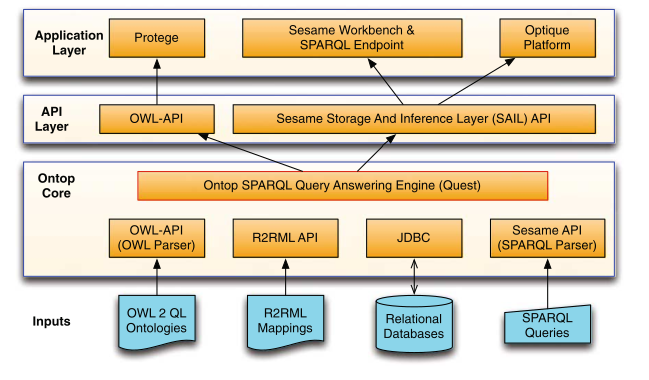
\includegraphics[width=0.75\linewidth]{OntopArchitecture.png}
    \caption{Struttura di Ontop}
    \label{fig:OntopArchitecture}
\end{figure}

\subsection{Intermediate Query language}
\label{sec:ontop_iq}
Ontop era inizialmente basato su Datalog come motore interno per la traduzione delle query. Questo è però risultato essere insufficiente per permettere la traduzione di un frammento più grande di SPARQL 
che supporta funzionalità non monotone come OPTIONAL, modificatori di cardinalità come DISTINCT e aggregazione che non possono essere espresse come unione di query congiuntive (UCQ). Per questo con la versione
v4 Ontop ha adottato uan struttura dati interna diversa chiamata Intermediate Query (IQ) che fornisce una rappresentazioni uniforme sia per le query SPARQL eseguite dagli utenti che per le query SQL dei mapping.
Sostanzialmente un IQ è una rappresentazione tramite un albero radicato di un'espressione algebrica dove quest'algebra è un compromesso tra l'algebra di SPARQL da una parte e l'algebra relazionale tipica dei database 
relazionali dall'altra.

Prima di definire più nel dettaglio quest'algebra è necessario spiegare alcuni altri termini e in particolare:
\begin{itemize}
    \item termine: per termine indichiamo qualsiasi variabile, costante (incluso NULL) o termine funzionale costruito a partire da variabili o costanti usando simboli funzionali di SPARQL, SQL o interni
    \item sostituzione: per sostituzione intendiamo un'espressione della forma \linebreak
        $x_1/\mu_1 , \dots , x_n/\mu_n $ dove $x$ corrisponde ad una variabile e $\mu$ ad un termine usato o per la proiezione o per l'aggregazione.
\end{itemize} \cite{Ontop}

I nodi che compongono questo albero IQ possono essere:
\subsubsection*{Nodi foglia} 
Tra i nodi che compongono le foglie dell'albero i più interessanti sono:
    \begin{itemize}
        \item intensional data node: node prototipo che si ci aspetta venga sostituito da un IQ ed è usato principlamente per rappresentare triple e quadruple RDF
        \item extensional data node: simile a un intensional data node con la differenza che non deve essere necessariamente essere sostituito (ad esempio se rappresenta il nome di una tabella)
        \item empty node: può essere visto come uno specifico tipo di data node che rappresenta un insieme vuoto di tuple
        \item true node: 
        \item native node
        \item values node
    \end{itemize}
\subsubsection*{Nodi interni} 
I nodi interni dell'albero risultano essere più interessanti rispetto alle foglie in quanto rappresentano quelle che sono le operazioni possibili e che devono essere tradotte tra SPARQL e SQL. Tra queste abbiamo:
    \begin{itemize}
        \item filter node: filtra il proprio nodo figlio in base ad una condizione
        \item inner join node: natural join tra gli n figli del nodo sui quali può anche essere applicata una condizione booleana di join
        \item left join node: rappresentazione di left outer join tra i due figli del nodo eventualmente con condizione di join
        \item union node: unione degli n figli
        \item construction node: rappresenta la sequenza di una proiezione seguita da un opzionale rinomina
        \item aggregation node: definito dall'insieme di variabili su cui viene eseguita l'aggregazione e una sostituzione per definire le nuove variabili ricavate dalle funzioni di aggregazione
        \item slice node: contiene un limite e/o un offset usati per eliminare un certo numero di tuple dal risultato
        \item distinct node: mantiene una singola occorrenza per ogni tupla
        \item order by node: ordine le tupe presenti in base ad una lista di comparatori. I valori vengono ordinati in base al primo comparatore e, solo in caso di valori uguali, viene usato il secondo comparatore e così via
            L'operatore segue una semantica NULL FIRST ASC / NULL LAST DESC 
    \end{itemize} \cite{IQ}

\begin{comment}
Formalmente quest'algebra è definita come:
\begin{equation}
    \begin{split}
        \phi := &P(t) \ | \ PROJ_\tau^x \ \phi \ \ | \ AGG_\tau^x \ \phi \ \ | \  DISTINCT \ \phi \ \ | \ ORDERBY_x \ \phi \ \ | \\
                &SLICE_i,j \ \phi \ \ |\ FILTER_\beta \ \phi \ \ | \ JOIN_\beta (\phi_1, \dots, \phi_k ) \ | \\
                &LEFTJOIN_\beta(\phi_1, \phi_2) \ | \ UNION(\phi_1, \dots, \phi_k ) 
    \end{split}
\end{equation}
dove $P$ è il nome di una relazione, $t$ è una tupla di termini, $x$ è una tupla di variabili, $\tau$ è una sostituzione, $i,j$ sono numeri naturali che descrivono il limite e l'offset e $\beta$ è un termine booleano.
\end{comment}
    
Nonostante la maggior parte del processamento della query sia poi lasciato al DBMS (Ontop modella ogni dialetto individualmente usando Java factory specifiche per ogni dialetto), IQ si occupa di tradurre aspetti della query SPARQL nel loro equivalente SQL. Questo è scontato per alcuni costrutti dove sia sintassi che 
semantica sono consistenti, mentre per altri i due linguaggi hanno comportamenti diversi. Di seguito si elencano alcune delle differenze principali tra i due linguaggi: \cite{Ontop}
\begin{itemize}
    \item tipizzazione: SQL è staticamente tipizzato ovvero tutti i valori in una colonna devono essere dello stesso tipo mentre SPARQL usa tipi dinamici. Questo significa che in SPARQL una funzione può accettare tipi diversi mentre questi
        sono fissi in SQL (ad esempio numeric\_add)
    \item ordinamento: SPARQL deve definire un ordine predefinito per IRI, blank nodes, variabili e letterali mentre in SQL è solamente necessario scegliere il modificato e specificare l'rodine per NULL
    \item condizione di join: al fine di effettuare un join in SPARQL i due mapping devono essere compatibili ovvero devono condividere la stessa variabile o lo stesso termini RDF (e quindi hanno la stesso tipo e valore lessicale). Per quanto 
        riguarda SQL invece non è necessario che gli argomenti siano dello stesso tipo e possono anche avere valori lessicali diversi (ad esempio timestamps con diversi fusi orari)
    \item dialetti: mentre SPARQL ha sintassi e semantica standard, SQL è vendor-specific 
\end{itemize}
In particolare Ontop modella ogni dialetto individualmente usando Java factory specifiche per ogni dialetto ovvero modella i tipi, le convenzioni nei nomi di attributi e tabelle, la semantica delle funzioni, la struttura dei data catalog, \dots individualmente per ogni dialetto. 

\subsection{Esempi di utilizzo}
Data la distribuzione di Ontop come progetto open-source con licenza Apache2 è impossibile conoscerne tutti i casi di utilizzo. Nonostante ciò esistono comunque casi documentati di uso di questo VGK system sia in ambito commerciale che pubblico.
\subsubsection*{Open Data Hub-Virtual-Knowledge-Graph}
Open Data Hub-Virtual Knowledge Graph nasce come un progetto congiunto tra il NOI Techpark e Ontopic al fine di pubblicare e rendere disponibili i dati del'Alto Adige su turismo e mobilità. Inizialmente questi dati erano accessibili attraverso un'API JSON, ma l'introduzione di un VKG, con annesso endopoint SPARQL, ha
reso questo sistema estremamente più potente e flessibile.
\subsubsection*{UNiCS}
UNiCS è una piattaforma sviluppata da SIRIS Academin che integra dati provenienti fonti come la commissione europea, governi nazionali e regionali e specifiche università al fine di aiutare università ed istituti di ricerca nel prendere scelta informate. Tutti questi dati sono disponibili tramite un'ontologia che può 
essere interrogata tramite un endpoint SPARQL e i risultati possono poi essere visualizzati tramite grafiche e statistiche di più facile interpretazione \cite{UniCS}.


\chapter{Progetto}
\label{cha:experience}

\section{Ontopic}
\label{sec:ontopic}
Il tirocinio da me svolto è avvenuto presso l'azienda Ontopic s.r.l. Tale azienda è nata nel 2019 come spin-off della Libera Università di Bolzano dal prof. Diego Calvanese insieme al professore Marco Montali, i ricercatori Guohui Xiao e Benjamin Cogrel
e l’amministratore delegato Peter Hopfgartner presso il NOI Techpark di Bolzano\cite{Ontopic}.

L'azienda nasce con lo scopo di proporre soluzioni di data integration ed in particolare basate sull'integrazione semantica come i Virtual Knowledge Graph. Ontopic fornisce sia consulenza diretta ad aziende con soluzioni ad-hoc
per integrazione ed analisi dati che una soluzione proprietaria per il mapping di VKG chiamata Ontopic Studio. Questo applicativo è basato sul Knowledge Graph system Ontop, di cui Ontopic è uno dei principali contributori, e permette di realizzare mapping
in modo efficiente tramite un interfaccia grafica no-code semplice che ne permette quindi l'uso anche a persone senza un background in tecniche semantiche. \cite{OntopicStudio}

\section{Il modulo bi-connector}
\label{sec:bi-connector}
Durante la mia esperienza di tirocinio presso Ontopic, ho lavorato all'interno del progetto del bi-connector. Tale modulo ha lo scopo di permettere all'utente finale di ricavare informazioni su un VKG non solo tramite query SPARQL, come di consuetudine, ma anche
tramite strumenti di Business Intelligence (BI) come Tableau, PowerBi o Qlik.
Mentre questi applicativi presentano nativamente connettori verso molteplici fonti di dati tra cui: la maggior parte dei database relazionali, database NoSQL come MongoDB, fogli Excel,
dati in formato JSON, file PDF, connessioni personalizzate tramite JDBC o ODBC, \dots, non forniscono invece connettori nativi per i VKG ed è proprio per questo che nasce bi-connector.

\begin{comment}{}
In particolare, il primo applicativo di business intelligence su quale si è focalizzato lo sforzo di sviluppo è stato Tableau e perciò nel resto dell'elaborato farò principalmente riferimento a questo.
\end{comment}
Possiamo pensare a bi-connector come costituito di due parti principali: una che si occupa della costruzione di un database a partire dall'ontologia che possa essere connesso al strumento di BI target e una seconda parte che ha il compito di tradurre le query
SQL sul database in una forma comprensibile dal VKG sottostante.

\subsection{Creazione database}
\label{sec:bi-connector_db}
Dalle sorgenti di dati e dai file che utilizzati per creare i mapping di un VKG viene creato un database PostgreSQL.
Questo è reso possibile modificando direttamente i cataloghi di sistema resi disponibili da PostgreSQL tramite l'insieme di tabelle \textit{pg\_catalog}.
La comunicazione da e verso questo database è resa possibile tramite un'implementazione basata sul protocollo Wire che è il protocollo usato da PostgreSQL per lo scambio di messaggi.

Da estendere chiedendo a Benjamin

\subsection{Parsing di query SQL}
\label{sec:bi-connector_parsing}
\`E possibile interrogare il database inizialmente creato tramite query SQL, ma queste devono poi essere tradotte in una rappresentazione comprensibile dal VKG sottostante. Questo perché le query non sono eseguite sul database da noi creato, ma sul
Virtual Knowledge Graph originale così da poterne sfruttare le capacità di inferenza.

In quanto il VKG system utilizzato è Ontop, le query SQL vengono tradotte in un albero IQ, descritto precedentemente anche nella sezione \ref{sec:ontop_iq}.

Inizialmente, le query delle quali era possibile fare il parsing erano quasi esclusivamente del tipo SELECT-JOIN-WHERE, ovvero un'unione di query congiuntive. Questo era dovuto al fatto che il parser SQL in uso era quello nativo di Ontop,
il quale ha come scopo principale la traduzione dei mapping che sono, nella maggior parte dei casi, rappresentabili tramite questo tipo di semplici query.
A causa di questa limitazione moltissime delle query generate automaticamente da strumenti di Business Intelligence dovevano essere riscritte in una forma semplifica per poter essere eseguite.
Di seguito un esempio di ciò in cui la query è semplificata eliminando il LEFT JOIN e l'ORDER BY in quanto non supportati.
\begin{verbatim}
    SELECT n.oid, n.*, d.description 
    FROM pg_catalog.pg_namespace n
    LEFT OUTER JOIN pg_catalog.pg_description d ON d.objoid=n.oid 
        AND d.objsubid=0 AND d.classoid='pg_namespace'::regclass
    ORDER BY nspname
diventa:
    SELECT n.* 
    FROM pg_catalog.pg_namespace n;
\end{verbatim}

Date queste limitazioni del parser originale, si è deciso di adottarne uno diverso ovvero JSqlParser. JSqlParser è un parser di istruzioni SQL
che trasforma una query in una gerarchia di classi Java. \`E basato sul visitor pattern il quale permette di separare in modo semplice un algoritmo dalla struttura dati sulla quale è utilizzato.
In particolare tale pattern rappresenta un'operazione che deve essere eseguita su un insieme eterogeneo di oggetti e, per ognuno di questi, potrebbe dover essere implementata in modo differente \cite{JSqlParser}.

\section{Prime attività}
\label{sec:prerequisits}
La prima attività svolta all'interno del tirocinio è stata quella di familiarizzare con le tecnologie legate ai VKG che mi sarebbero servite in seguito. In particolare ho svolto
il tutorial introduttivo ad Ontop tramite la piattaforma Protege così da provare direttamente cosa si intende per tradurre fonti di dati in un'ontologia tramite mapping. (Forse non mettere)

Il mio compito principale è stato quello di estendere il parser SQL in uso così da supportare un numero maggiore di costrutti. Come affermato anche precedentemente, il parser inizialmente utilizzato era
esclusivamente in grado di tradurre semplici query il che è risultato essere insufficiente affinché potesse essere usato da strumenti di Business Intelligence in modo non banale.

\`E stato quindi analizzato quali fossero i costrutti maggiormente presenti nelle query generate automaticamente dagli strumenti di BI, di cui un esempio sopra nella sezione \ref{sec:bi-connector_parsing}. Tra questi
i principali erano sicuramente il GROUP BY per l'aggregazione, dato anche lo scopo degli strumenti di BI di fornire informazioni riassuntive d'insieme sull'intero dataset, e l'ORDER BY che
permette di visualizzazione i dati in base a parametri arbitrari.

\subsection{Database di riferimento}
Durante la durata del tirocinio, tutte le funzionalità implementate sono state testate su un semplice VKG con un database relazionale H2 come sorgente che rappresenta alcune informazioni riguardanti professori universitari.
I test sono stati eseguiti sia all'interno della codebase stessa grazie al framework JUnit che tramite il client SQL DBeaver che ha permesso la visualizzazione del database PostgreSQL creato dal bi-connector e la sua
interrogazione diretta.
Di seguito si descrivono le tabelle (\ref{tab:prof} \ref{tab:profstats}, \ref{tab:course}, \ref{tab:teaching}) di questo database che sono inoltre quelle a cui si farà riferimento in tutti i frammenti di codice successivi.
\begin{table}
    \caption{Tabella prof}
    \label{tab:prof}
    \centering
    \begin{tabular}{ | c | c | c | }
        \hline
        id                                         & fName   & lName   \\ \hline
        http://university.example.org/professor/10 & Roger   & Smith   \\ \hline
        http://university.example.org/professor/20 & Frank   & Pitt    \\ \hline
        http://university.example.org/professor/30 & John    & Deep    \\ \hline
        http://university.example.org/professor/40 & Micheal & Jackson \\ \hline
        http://university.example.org/professor/50 & Diego   & Gamper  \\ \hline
        http://university.example.org/professor/60 & Johann  & Helmer  \\ \hline
        http://university.example.org/professor/70 & Barbare & Dodero  \\ \hline
        http://university.example.org/professor/80 & Mary    & Poppins \\ \hline
    \end{tabular}
\end{table}

\begin{table}
    \caption{Tabella prof\_stats}
    \label{tab:profstats}
    \centering
    \begin{tabular}{| c | c | c |}
        \hline
        profId                                     & totalStudents & countCourse \\ \hline
        http://university.example.org/professor/10 & 21            & 2           \\ \hline
        http://university.example.org/professor/30 & 12            & 1           \\ \hline
        http://university.example.org/professor/80 & 13            & 1           \\ \hline
    \end{tabular}
\end{table}

\begin{table}
    \caption{Tabella course}
    \label{tab:course}
    \centering
    \begin{tabular}{| c | c | c |}
        \hline
        id                                                       & duration & nbStudents \\ \hline
        http://university.example.org/course/LinearAlgebra       & 24.5     & 10         \\ \hline
        http://university.example.org/course/DiscreteMathematics & 30       & 11         \\ \hline
        http://university.example.org/course/AdvancedDatabases   & 20       & 12         \\ \hline
        http://university.example.org/course/ScientificWriting   & 18       & 13         \\ \hline
    \end{tabular}
\end{table}

\begin{table}
    \small
    \caption{Tabella teaching}
    \label{tab:teaching}
    \centering
    \begin{tabular}{| c | c | }
        \hline
        teacher                                    & course                                                   \\ \hline
        http://university.example.org/professor/30 & http://university.example.org/course/AdvancedDatabases   \\ \hline
        http://university.example.org/professor/10 & http://university.example.org/course/DiscreteMathematics \\ \hline
        http://university.example.org/professor/10 & http://university.example.org/course/LinearAlgebra       \\ \hline
        http://university.example.org/professor/80 & http://university.example.org/course/ScientificWriting   \\ \hline
    \end{tabular}
\end{table}
Inoltre, dato il fatto che ogni DBMS tende ad avere un proprio dialetto SQL, è stato molto importante assicurarsi che i costrutti da me implementati ricalcassero il
comportamento presente in PostgreSQL e, nel caso ciò non fosse possibile, fornire messaggi d'errore di facile comprensione. Ad esempio, la funzione \textit{concat()}
è null-rejecting, ovvero tutti gli argomenti pari a NULL sono ignorati, mentre in altri dialetti, come ad esempio MySQL, se uno degli argomenti è NULL allora il risultato
della concatenazione è anch'esso NULL.
Al fine di ottenere ciò, ho utilizzato la documentazione di PostgreSQL e, per test più pratici, ho usato DBFiddle, uno strumento online per testare in modo veloce, e
senza bisogno di alcun setup, frammenti di codice SQL.


\section{Costrutti implementati}
\label{sec:implementation}
La struttura usata per il parsing è basata sulla classe \textit{IQTreeExpression.java} la quale è composta da:
\begin{itemize}
    \item IQTree: albero composto di nodi IQ che viene costruito partendo dalle foglie e viene esteso aggiungendo nuovi nodi come radici dell'albero stesso. Da un punto di vista
          più pratico abbiamo come foglie degli extensional node che rappresentano le tabelle elencate all'interno della query e al di sopra di esse sono presenti altri nodi che
          rappresentano le varie operazioni eseguite.
    \item RAExpressionAttributes: dizionario che contiene le colonne delle tabelle coinvolte nella query e tutti gli alias ad esse associati. Per alias si intendono i nomi definiti
          dall'utente tramite la keyword AS o come nome di una tabella e quelli definiti internamente al codice al fine di assicurarne l'univocità.
\end{itemize}
Di seguito un esempio di un IQTreeExpression generato dalla query
\begin{verbatim}
    SELECT "id", "fName", "lName"
    FROM prof p

    IQTreeExpression{
        iqTree = EXTENSIONAL "prof_views"."prof"(0:id1,1:fName1,2:lName1), 
        raExpressionAttributes=attributes: {"id"=id1, p."id"=id1, 
         "fName"=fName1, p."fName"=fName1, "lName"=lName1, p."lName"=lName1} 
         with {"id"=[p], "fName"=[p], "lName"=[p]}
    } 
    \end{verbatim}

\subsection{Modificatori di cardinalità}
I primi costrutti da essere implementati sono stati quelli responsabili della modifica della cardinalità di una tabella ovvero DISTINCT e LIMIT-OFFSET. La loro implementazione
risulta essere abbastanza semplice da un punto di vista logico, ma ciò mi ha permesso di acquisire familiarità con la codebase preesistente e con librerie esterne come JSqlParser
in modo più rapido dato che l'implementazione dei costrutti non aveva logiche complesse.

\subsubsection*{DISTINCT}
Il costrutto DISTINCT permette di eliminare righe duplicate ed è stato implementato aggiungendo un nodo IQ di tipo distinct.

La clausola DISTINCT ON non è stata invece implementata in quanto non parte dello standard SQL, ma fornita da PostgreSQL. Inoltre non è stata considerata fondamentale in quanto
può essere rimpiazzata tramite l'uso di una subquery o in alcuni casi anche tramite aggregazione \cite{PGDistinct}.
\subsubsection*{LIMIT e OFFSET}
Le clausole LIMIT e OFFSET permettono di restringere il numero di righe restituite da una query e di saltare le prime $n$ righe quando queste vengono restituire rispettivamente.
Data le loro funzionalità complementari sono spesso usate insieme anche se è possibile usare singolarmente
Ad esempio la forma \verb+LIMIT 5 OFFSET 2+ ritorna le prime 5 righe dopo che sono state saltate le prime 2.

Anche se supportata dalla maggior parte dei DBMS, e quindi ampiamente usata, la clausola LIMIT non fa parte dello standard SQL. Una possibile alternativa standardizzata è l'utilizzo
della keyword FETCH la cui sintassi è \verb+FETCH { FIRST | NEXT } [ fetch_rows ] { ROW | ROWS }+ \verb+ONLY+ dove FIRST/NEXT e ROW/ROWS sono sinonimi e possono quindi essere usati
in modo intercambiabile \cite{Fetch}.

Al fine di implementarne la funzionalità, indipendentemente se per LIMIT o per FETCH, è stato usato uno slice node il quale permette di specificare esclusivamente un offset o sia
un limite che un offset.

Inoltre, quando si utilizza LIMIT è consigliato aggiungere anche un ORDER BY che forza un ordine alle righe altrimenti il risultato non è garantito che il risultato sia lo stesso per
esecuzioni successive della stessa query \cite{PGLimit}.

\subsection{Ordinamento righe}
La keyword ORDER BY permette riordinare le righe risultanti da una query in base a specifiche condizioni, sia in modo ascendente che discendente. Un altro aspetto importante è quello del
NULL ordering, ovvero come i valori NULL sono trattati al fine dell'ordinamento. In PostgreSQL i valori pari a NULL vengono considerati come maggiori di qualsiasi altro valore mentre questo
è l'opposto per gli IQ tree i quali seguono una semantica simile a quella di SPARQL. Quindi gli ordinamenti del tipo \verb+ORDER BY ASC NULLS LAST+ e \verb+ORDER BY DESC NULLS FIRST+
non sono supportati \cite{PGOrderBY}.

L'implementazione dell'ORDER BY è risultata essere relativamente complessa in quanto può essere usata su un'ampia casistica. Ad esempio si può avere uno o più criteri di ordinamento e
ognuno di essi può essere una colonna o una funzione. Inizialmente il costrutto è stato implementato usando un order by node il quale richiede come argomento una lista di comparatori
dove ogni comparatore è costituito dal termine rispetto al quale si sta effettuando l'ordinamento e se quest'ultimo è ascendente o meno.

Una volta svolti i primi test, è subito emerso un problema riguardante la rinomina delle variabili in quanto una volta che ad una variabile veniva assegnato un alias si andava a perdere
quale fosse il nome della variabile originale. Quindi ad esempio un query del tipo:
\begin{verbatim}
    SELECT "fName" as v
    FROM prof p 
    ORDER BY "fName"
\end{verbatim}
avrebbe restituito un errore in quanto l'unica variabile presente a seguito della proiezione sarebbe stata \textit{v} e sarebbe quindi stato impossibile eseguire un ordinamento basato su
\textit{fName}.

Si è quindi deciso di estendere l'implementazione per supportare questo comportamento aggiungendo un construction node che proietta tutte le variabili e tiene traccia delle sostituzioni che
avvengono. Inoltre al fine di evitare collisioni tra gli attributi non proiettati, che vengono appunto mantenuti in questa versione, e gli alias, tutti gli attributi sono rinominati aggiungendo un
suffisso casuale al nome della variabile stessa. La query vista sopra produce questa IQTreeExpression:
\begin{verbatim}
    IQTreeExpression{
        iqTree=CONSTRUCT [v] []
         ORDER BY [ASC(fName)]
          CONSTRUCT [v, fName, fName1f1611f1-6d9d-4347-9c60-f51bbdc89a09, 
            lName, lName0c931a3d-93fb-406c-b33c-6f4743af211c, id, 
            idf859a5d9-d246-42a2-a62f-e722a1175dc4] [fName/v, 
            idf859a5d9-d246-42a2-a62f-e722a1175dc4/id, 
            lName0c931a3d-93fb-406c-b33c-6f4743af211c/lName, 
            fName1f1611f1-6d9d-4347-9c60-f51bbdc89a09/v]
           CONSTRUCT [id, v, lName] []
            EXTENSIONAL "prof_views"."prof"(0:id,1:v,2:lName), 
        raExpressionAttributes=attributes: {v=v} with {v=[]}
    } 
\end{verbatim}

\`E inoltre possibile una forma del tipo \verb+ORDER BY numerical_constant+ dove la costante numerica presente viene utilizzata come indice della corrispondente colonna proiettata. Tale
uso è scoraggiato in quanto il risultato potrebbe non essere deterministico se si va a cambiare la struttura del database stesso, ma è stato implementato ugualmente in quanto viene
ampiamente usato nelle query generate in modo automatico da Tableau.

\subsection{Combinazione tabelle}
Un'altra parte importante al fine formulare query con risultati non banali, è la possibilità di combinare le informazioni presenti in molteplici tabelle. Personalmente, mi sono occupata
esclusivamente dell'implementazione del LEFT JOIN in quanto CROSS e INNER JOIN erano già entrambi funzionanti nel momento in cui ho iniziato il mio tirocinio.

In particolare, l'operazione di LEFT JOIN estende tutte le righe della prima tabella con i valori di una seconda tabella basandosi su una determinata condizione booleana di join. Tale condizione
può essere espressa in due modi:
\begin{itemize}
    \item \verb+LEFT JOIN ON condition+: in questo caso viene specificata una serie di condizioni, tipicamente di uguaglianza tra due colonne appartenenti a tabelle diverse
    \item \verb+LEFT JOIN USING column+: usato se la colonna rispetto alla quale vogliamo eseguire il join ha lo stesso nome in entrambe le tabelle
\end{itemize}

A fini implementativi, entrambe le condizioni vengono espresse come un ImmutableExpression, ovvero un espressione booleana, la quale viene usata come filtro all'interno di un left join node.
Di seguito un esempio dell'IQTreeExpression e del risultato generato dalla query:
\begin{verbatim}
    SELECT p.id, "fName", "totalStudents"
    FROM prof p
    LEFT JOIN prof_stats ps ON p.id = ps."profId"
\end{verbatim}
la quale produce come IQTreeExpression
\begin{verbatim}
    IQTreeExpression{iqTree=CONSTRUCT [id, fName, totalStudents] []
     CONSTRUCT [id, fName, totalStudents,lName, countCourse, profId,
        variabili generate casualmente per univocità] [elenco 
        sostituzioni come visto precedentemente]
      CONSTRUCT [id, fName, lName, profId, totalStudents, countCourse] []
       LJ STRICT_EQ2(id,profId)
        EXTENSIONAL "prof_views"."prof"(0:id,1:fName,2:lName)
        EXTENSIONAL "prof_views"."prof_stats"(0:profId,1:totalStudents,
            2:countCourse), 
    raExpressionAttributes=attributes: {id=id, "fName"=fName, 
        "totalStudents"=totalStudents} with {id=[], "fName"=[], 
        "totalStudents"=[]}}
\end{verbatim}
ed ha come risultato la tabella \ref{tab:leftJoinOn}.
\begin{table}[ht]
    \centering
    \caption{Tabella LEFT JOIN}
    \label{tab:leftJoinOn}
    \begin{tabular}{ | c | c | c | c | c | c |}
        \hline
        id                                         & fName   & totalStudents \\ \hline
        http://university.example.org/professor/10 & Roger   & 21            \\ \hline
        http://university.example.org/professor/20 & Frank   & NULL          \\ \hline
        http://university.example.org/professor/30 & John    & 12            \\ \hline
        http://university.example.org/professor/40 & Micheal & NULL          \\ \hline
        http://university.example.org/professor/50 & Diego   & NULL          \\ \hline
        http://university.example.org/professor/60 & Johann  & NULL          \\ \hline
        http://university.example.org/professor/70 & Barbare & NULL          \\ \hline
        http://university.example.org/professor/80 & Mary    & 13            \\
        \hline
    \end{tabular}
\end{table}

Questa implementazione risulta non essere però completa in quanto presenta comportamenti non corretti in alcuni casi nei quali le colonne sulle quali viene eseguito il join hanno lo stesso nome.
Ad esempio, la query
\begin{verbatim}
    SELECT p.*, ps.*
    FROM (SELECT id as "profId", "fName", "lName" FROM prof_views.prof p1) p
    LEFT JOIN prof_views.prof_stats ps ON p."profId" = ps."profId"
\end{verbatim}
ritorna un errore in quanto i nomi di due colonne all'interno del SELECT sono uguali. Questa è una limitazione di Ontop stesso il quale non permette di avere variabili
con lo stesso nome all'interno di una proiezione.

Una volta realizzato il LEFT JOIN, l'implementazione del RIGHT JOIN è risultata essere banale in quanto è sufficiente invertire i ruoli delle due tabelle sulle quali viene effettuato
il join per ottenere il comportamento corretto.

\subsection{Operazioni insiemistiche}
Gli operatori insiemistici uniscono i risultati di due query in un unico insieme finale. I due insiemi che devono essere uniti devono rispettare alcune condizioni:
devono restituire lo stesso numero di colonne e colonne corrispondenti devono avere tipi compatibili \cite{PGSetOp}. Inoltre, una limitazione aggiuntiva introdotta dalla nostra
implementazione prevede che colonne corrispondenti debbano avere lo stesso nome.

\subsubsection*{UNION}
L'operazione di UNION aggiunge alle righe risultanti dalla prima query quelle ottenute da una seconda query eliminando i duplicati. Se si vuole mantenere le righe duplicate è possibile
usare il costrutto UNION ALL.

La sua implementazione prevede l'utilizzo di uno union node, il quale mantiene i duplicati, seguito eventualmente da un distinct node nel caso sia necessario eliminare le copie.

\subsubsection*{EXCEPT}
L'operazione di sottrazione, chiamata in PostgreSQL EXCEPT invece dello standard MINUS, restituisce tutte le righe risultanti dalla prima query che non sono presenti anche nei
risultati della seconda.

La sua implementazione risulta essere particolarmente interessante in quanto non esiste un IQ node che ne imiti di comportamento. Viene quindi eseguito un left join tra le due
tabelle e tramite un filtro vengono eliminate tutte le righe per le quali le colonne provenienti dalla tabella di destra, identificate dalla colonna ausiliaria \textit{rightProv},
non sono pari a NULL. Infine viene usato un construct node così da mantenere solo le variabili desiderate. Ad esempio la query
\begin{verbatim}
    SELECT "id"
    FROM prof p
    EXCEPT
    SELECT "profId" AS "id"
    FROM prof_stats ps 
\end{verbatim}
ha come risultato la tabella \ref{tab:minus}
\begin{table}[h]
    \centering
    \caption{Tabella MINUS}
    \label{tab:minus}
    \begin{tabular}{ | c | c | c | c | c | c |}
        \hline
        id                                         \\ \hline
        http://university.example.org/professor/20 \\ \hline
        http://university.example.org/professor/40 \\ \hline
        http://university.example.org/professor/50 \\ \hline
        http://university.example.org/professor/60 \\ \hline
        http://university.example.org/professor/70 \\
        \hline
    \end{tabular}
\end{table}

\noindent
e produce come l'IQTreeExpression:
\begin{verbatim}
    IQTreeExpression{iqTree=CONSTRUCT [id] []
     FILTER IS_NULL(rightProv)
       LJ
        CONSTRUCT [id] []
         CONSTRUCT [id, fName, lName, variabili generate casualmente per
          univocità] [elenco sostituzioni]
            CONSTRUCT [id, fName, lName] []
             EXTENSIONAL "prof_views"."prof"(0:id,1:fName,2:lName)
        CONSTRUCT [id, rightProv] [rightProv/"TRUE"^^BOOLEAN]
         CONSTRUCT [id] []
          CONSTRUCT [id, totalStudents,countCourse, variabili generate 
           casualmente per univocità] [elenco sostituzioni]
            CONSTRUCT [id, totalStudents, countCourse] []
             EXTENSIONAL "prof_views"."prof_stats"(0:id,1:totalStudents,
             2:countCourse),
    raExpressionAttributes=attributes: {"id"=id} with {"id"=[]}}
\end{verbatim}

Inoltre non è stato possibile implementare l'operazione di EXCEPT ALL in quanto non supportata dalla versione in uso di JSqlParser.

\subsection{Aggregazione}
L'aggregazione è una funzionalità estremamente importante in quanto permette di raggruppare i dati in base a parametri arbitrari ed
ottenere da questi informazioni riassuntive sui dati.
\subsubsection*{Funzioni di aggregazione}
Le funzioni di aggregazione (SUM, COUNT, MIN, MAX, AVG ) permettono di esprimere caratteristiche di una colonna, o di un'intera tabella,
tramite un singolo numero riassuntivo.

Il principale ostacolo alla loro implementazione è stato il determinare il tipo della colonna sulla quale la funzione era applicata.
Per questo, inizialmente, si è assunto a priori che tutte le funzioni di aggregazione fossero eseguite su colonne di tipo intero. In un
secondo momento si è implementato un meccanismo grazie alla classe
\textit{NotYetTypedAggregationFunctionSymbol.java} la quale permette di posporre la decisione sul tipo di dato fino a quando questo non è
reso disponibile.

Ad esempio, le due query seguenti applicano la funzione SUM alle colonne nbStudents e duration le quali sono rispettivamente un numero intero
e uno decimale ed è possibile vedere ciò nel tipo che viene dato alla funzione all'interno dell'aggregation node.
\begin{verbatim}
    SELECT sum("nbStudents") AS sum
    FROM course c 
\end{verbatim}
produce l'IQTreeExpression:
\begin{verbatim}
    IQTreeExpression{iqTree=CONSTRUCT [sum] []
     CONSTRUCT [sum] []
      AGGREGATE [] [sum/SUM_BIGINT(nbStudents1)]
       CONSTRUCT [id1, duration1, nbStudents1] []
        EXTENSIONAL "prof_views"."course"(0:id1,1:duration1,2:nbStudents1),
    raExpressionAttributes=attributes: {sum=sum} with {sum=[]}}
\end{verbatim}
mentre la query
\begin{verbatim}
    SELECT sum("duration") AS sum
    FROM course c 
\end{verbatim}
produce l'IQTreeExpression
\begin{verbatim}
    IQTreeExpression{iqTree=CONSTRUCT [sum] []
     CONSTRUCT [sum] []
      AGGREGATE [] [sum/SUM_DECIMAL(duration1)]
       CONSTRUCT [id1, duration1, nbStudents1] []
        EXTENSIONAL "prof_views"."course"(0:id1,1:duration1,2:nbStudents1),
    raExpressionAttributes=attributes: {sum=sum} with {sum=[]}}    
\end{verbatim}

\subsubsection*{GROUP BY}
La clausola GROUP BY permette di raggruppare insieme righe di una tabella che hanno lo stesso valore per tutte le colonne per le quali stiamo 
raggruppando. Una volta avvenuto il raggruppamento determinati gruppi possono essere eliminati in base ad una condizione booleana
specificata all'interno del costrutto HAVING, in modo simile a quanto accade per la clausola WHERE \cite{PGGroupBy}.

Il costrutto viene implementato tramite un aggregation node al di sopra del quale viene aggiunto un filter node nel caso in cui sia presente 
la clausola HAVING. La parte più problematica risulta essere la gestione della proiezione degli variabili in quanto solo le variabili rispetto 
a cui si raggruppato possono essere proiettate, ma allo stesso tempo è necessario mantenere anche tutte le variabili rispetto a quali non si
è raggruppato in quanto queste possono essere usate all'interno di funzioni di aggregazione nel SELECT e nel HAVING. 

Inoltre il GROUP BY permette di raggruppare non solo in base a colonne nella tabella, ma anche con funzioni. Al fine di rendere l'implementazione
omogenea con il caso base descritto sopra, prima di gestire il GROUP BY viene aggiunto un construction node dove ogni funzione distinta presente 
viene sostituita con una variabile; in questo modo il GROUP BY "vede" esclusivamente variabili. 
Di seguito una query di esempio:
\begin{verbatim}
    SELECT teacher, MIN(course) AS "minCourse"
    FROM teaching t 
    GROUP BY teacher, LENGTH("teacher") 
    HAVING LENGTH(teacher) > 20
\end{verbatim}
la quale ha come risultato la tabella \ref{tab:groupBy}
\begin{table}[ht]
    \small
    \centering
    \caption{Tabella GROUP BY}
    \label{tab:groupBy}
    \begin{tabular}{| c | c | }
        \hline
        teacher                                    & course                                                   \\ \hline
        http://university.example.org/professor/10 & http://university.example.org/course/DiscreteMathematics \\ \hline
        http://university.example.org/professor/30 & http://university.example.org/course/AdvancedDatabases   \\ \hline
        http://university.example.org/professor/80 & http://university.example.org/course/ScientificWriting   \\ \hline
    \end{tabular}
\end{table}
e produce l'IQTreeExpression
\begin{verbatim}
    IQTreeExpression{iqTree=CONSTRUCT [teacher, minCourse] []
     CONSTRUCT [teacher, minCourse, teacher1c52a1c4-11f6-43c1-8311-9e908578b9] 
     [teacher1c52a1c4-11f6-43c1-8311-9e908578b9/teacher]
      FILTER GT(CHAR_LENGTH1(teacher),"20"^^BIGINT)
       AGGREGATE [fun6079a412-7f91-4004-9bcc-f3e2f545d3ce, teacher] 
       [minCourse/MIN_TEXT(course1)]
        CONSTRUCT [teacher, course1, fun6079a412-7f91-4004-9bcc-f3e2f545d3ce] 
        [fun6079a412-7f91-4004-9bcc-f3e2f545d3ce/CHAR_LENGTH1(teacher)]
         EXTENSIONAL "prof_views"."teaching"(0:teacher,1:course1),
    raExpressionAttributes=attributes:{teacher=teacher, "minCourse"=minCourse} 
    with {teacher=[], "minCourse"=[]}}
\end{verbatim}
Come detto prima è appunto possibile vedere il construction node al di sotto dell'aggregation node che esegue la sostituzione rispetto alla funzione
LENGTH e il filtro usato per l'implementazione del HAVING al di sopra dell'aggregation node.

Così come per l'ORDER BY, anche per il GROUP BY è possibile indicare le colonne rispetto a cui si vuole raggruppare utilizzando un indice numerico.

\section{Risultati ottenuti}
Con l'introduzione dei costrutti elencati fino ad adesso si è reso possibile la formulazione di query non banali. Ad esempio una query ,moderatamente
complessa, come quella descritta sotto può adesso essere tradotta correttamente.
\begin{verbatim}
    SELECT "teacher", sum("nbStudents") AS "totalStudents"
    FROM teaching t 
    LEFT JOIN course c on t.course = c.id 
    GROUP BY teacher 
    HAVING SUM(duration) >= 20
    ORDER BY teacher DESC
    LIMIT 1 OFFSET 1
\end{verbatim}
Questa query ritorna una singola riga \ref{tab:complex}
\begin{table}[ht]
    \small
    \centering
    \caption{Tabella riassuntiva}
    \label{tab:complex}
    \begin{tabular}{| c | c | }
        \hline
        teacher                                    & totalStudents  \\ \hline
        http://university.example.org/professor/10 & 21             \\ \hline
    \end{tabular}
\end{table}

\noindent
e genera come IQTreeExpression:
\begin{verbatim}
    IQTreeExpression{iqTree=SLICE offset=1 limit=1
     CONSTRUCT [teacher, totalStudents] []
      ORDER BY [DESC(teacher)]
       CONSTRUCT [teacher, teacher6be09e18-d526-4dd7-9447-c5dfa148ede7,
       totalStudents] [teacher6be09e18-d526-4dd7-9447-c5dfa148ede7/teacher]
        FILTER GTE(agg8dcab048-1be9-47d3-903e-fe401d8d21bd,"20"^^BIGINT)
         AGGREGATE [teacher] [totalStudents/SUM_BIGINT(nbStudents2), 
         agg8dcab048-1be9-47d3-903e-fe401d8d21bd/SUM_DECIMAL(duration2)]
          CONSTRUCT [teacher, course1, id2, duration2, nbStudents2] []
           LJ STRICT_EQ2(course1,id2)
            EXTENSIONAL "prof_views"."teaching"(0:teacher,1:course1)
            EXTENSIONAL "prof_views"."course"(0:id2,1:duration2,2:nbStudents2)
    raExpressionAttributes=attributes: {"teacher"=teacher, 
    "totalStudents"=totalStudents} with {"teacher"=[], "totalStudents"=[]}}
\end{verbatim}
Inoltre l'introduzione dell'aggregazione, e anche dell'ORDER BY, ha reso possibile l'accesso al database da parte di Tableau e la creazione delle prime 
dashboard.(chiedere a Benjamin se ha qualche screenshot)

\chapter{Conclusioni}
\label{cha:conclusions}
Il tirocinio presso Ontopic mi ha permesso di acquisire nuove competenze sia da un punto di vista puramente tecnico che 
personale. Infatti, per la prima volta ho avuto la possibilità di lavorare su del codice di livello aziendale dove 
l'affidabilità e leggibilità del codice implementato sono gli aspetti più importanti e, da un punto di vista più
pratico, approfondire le mie conoscenze in linguaggi quali Java e SQL. Inoltre ho potuto sperimentare in prima persona cosa significhi lavorare in un team di sviluppatori e come in esso 
vengano divise le responsabilità.

Un altro aspetto fondamentale che ha certamente contribuito all'esito positivo di quest'esperienza è sicuramente il 
mio interesse personale verso il mondo della data integration e dell'analisi dati. Durante questo 
tirocinio ho avuto infatti la possibilità di interfacciarmi con moltissime nuove tecnologie in questo campo come i Virtual Knowledge
Graph e tutti gli standard legati al semantic web (RDF, R2RML, SPARQL, \dots) ad essi associati.

\section{Possibili sviluppi futuri}
\label{sec:conclusions_future}
Il modulo bi-connector al quale ho lavorato durante tirocinio ha ampie potenzialità di crescita. Infatti, nonostante l'estensione
del parser SQL effettuata, moltissime funzionalità di SQL non sono implementate. Questo è particolarmente vero per quanto 
riguarda le funzioni: SQL presenta moltissime funzioni pre-implementate utili che non sono però supportate nel sistema,
come ad esempio buona parte delle funzioni per la manipolazione di date e fusi orari.

Inoltre è possibile allargare il supporto ad altri strumenti di Business Intelligence come ad esempio PowerBI o Qlik. Infatti, 
a seguito della fine del mio tirocinio, si è già iniziato a lavorare per estendere il supporto a PowerBI.



%bibliografia
\bibliographystyle{plain}
\bibliography{bibliography.bib}
\addcontentsline{toc}{chapter}{Bibliografia}
\end{document}